\section{Digital-Analog-Wandler (ADC)}
\todo{Woche 4 12.10.21}
\subsection{Parallelverfahren (Voltage Scalung)}
Quantisierungsschritt wird bestimmt durch den grössten Widerstand.

\subsection{Wägeverfahren}
\includegraphics[width=\linewidth]{Images/wägeverfahren}
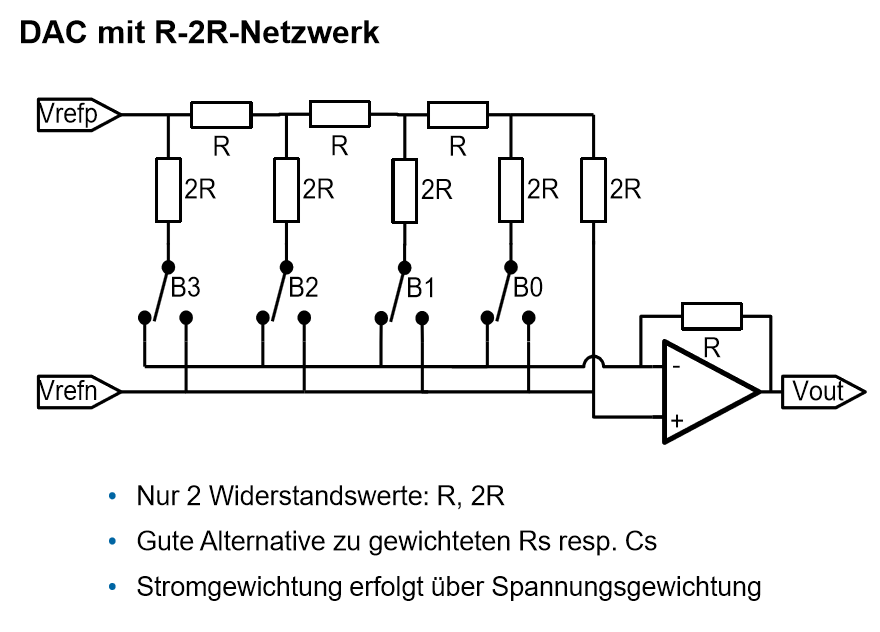
\includegraphics[width=\linewidth]{Images/r-2r}



\subsection{Zählverfahren}

\subsection{Eigenschaften}
\todo{Woche 5, 19.10.21}
\subsubsection{DAC Fehler}
\begin{enumerate}
	\item Offset-Fehler
	\item Verstärkungs-Fehler
	\item Integral Nichtlinearität INL
	\item Differentielle Nichtlinearität DNL
\end{enumerate}

\subsubsection{Verzögerungszeit, Settling Time}
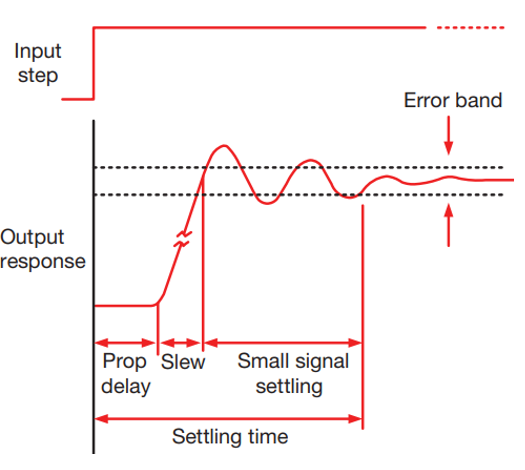
\includegraphics[width=0.4\linewidth]{Images/settling_imte}

